\documentclass{article}
\usepackage[utf8]{inputenc}
\usepackage{hyperref}
\usepackage[letterpaper, portrait, margin=1in]{geometry}
\usepackage{enumitem}
\usepackage{amsmath}
\usepackage{booktabs}
\usepackage{graphicx}
\usepackage{hyperref}
\usepackage{titlesec}

\hypersetup{
colorlinks=true,
    linkcolor=black,
    filecolor=black,      
    urlcolor=blue,
    citecolor=black,
}

  
\title{Economics 7103 - Homework 2}
\author{Ana Mazmishvili}
\date{ January 29, 2024 }
  
\begin{document}
  
\maketitle 

\section*{Python}
\textbf{Note:} \textit{I asked Afi to help me with the Python code only. That's why I will follow similar steps as he did with small modifications. }

\subsection*{Question 1.1}




\subsection*{Question 1.2}

\begin{figure}[ht]
    \centering
    \includegraphics[scale = 0.7]{}
    \caption{Kernel density plots of the electricity use for treated group and control group.}
    \label{fig:samplehist}
\end{figure}

\subsection*{Question 1.3}

\section*{Stata}

\subsection*{Question 2.1}


\begin{table}[ht]
    \centering
    {
\def\sym#1{\ifmmode^{#1}\else\(^{#1}\)\fi}
\begin{tabular}{l*{3}{c}}
\hline\hline
            &\multicolumn{1}{c}{Control}&\multicolumn{1}{c}{Treatment}&\multicolumn{1}{c}{P-value}\\
\hline
electricity &    1181.33 &    1086.75 &       0.001\\
            &   (454.31) &   (423.96) &     [3.404]\\
sqft        &    1633.05 &    1657.55 &       0.572\\
            &   (682.90) &   (686.27) &    [-0.566]\\
temp        &      79.89 &      79.89 &       0.987\\
            &     (2.16) &     (1.97) &    [-0.016]\\
\hline
Observations&         501&         499&       1,000\\
\hline\hline
\end{tabular}
}

    \caption{Summary statistics produced using Stata}
    \label{tab:my_label}
\end{table}

\subsection*{Question 2.2}

\begin{figure}[ht]
    \centering
    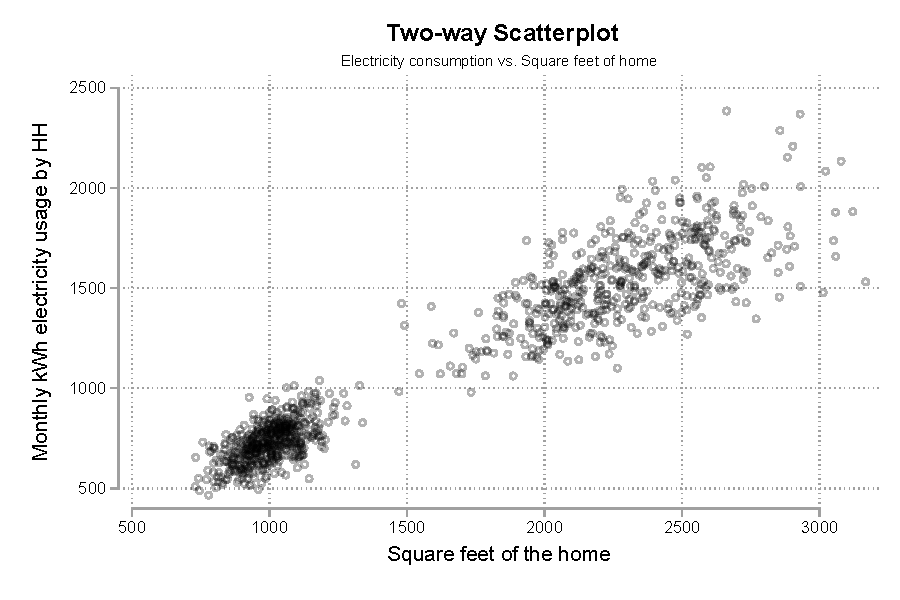
\includegraphics[scale = 0.7]{homework 2/output/figure/scatterplot.pdf}
    \caption{Scatterplot with electricity consumption and square feet of home}
\end{figure}

\subsection*{Question 2.3}
\begin{table}[ht]
    \centering
    \documentclass[]{article}
\setlength{\pdfpagewidth}{8.5in} \setlength{\pdfpageheight}{11in}
\begin{document}
\begin{tabular}{lc} \hline
 & (1) \\
VARIABLES & electricity \\ \hline
 &  \\
retrofit & -109.7*** \\
 & (7.943) \\
sqft & 0.615*** \\
 & (0.00678) \\
temp & 3.255* \\
 & (1.932) \\
Constant & -83.60 \\
 & (154.7) \\
 &  \\
Observations & 1,000 \\
 R-squared & 0.919 \\ \hline
\multicolumn{2}{c}{ Robust standard errors in parentheses} \\
\multicolumn{2}{c}{ *** p$<$0.01, ** p$<$0.05, * p$<$0.1} \\
\end{tabular}
\end{document}

    \caption{OLS regression results using Stata}
  \end{table}




\end{document}